\documentclass[12 pt,twoside]{article}
\usepackage{epsfig}
\usepackage{fullpage}
\usepackage[font={small,it}]{caption}

\begin {document}
\begin{center}

{\LARGE{\bf CCD Calibration Testing}}

{\large Tim Kornish}

University of Montana

October 20th, 2014
\end{center}
\paragraph{Abstract}

Testing the precision and accuracy of any Charge Coupled Device (CCD) is vital in analyzing images. CCD?s record digital images by counting electrons displaced by photons or photoelectrons. Complications of using a CCD arise from it not being able to distinguish photoelectrons from electrons given off by heat or any other reason. The CCD will be tested with bias images to remove counts not related to photoelectrons. Dark currents will also be tested with the CCD in complete darkness. Testing linearity of the CCD as exposure time increases the photon counts will increase at a linear rate. Testing the quantum efficiency of each of the 1024 X 1024 (approximately million) pixels. Testing the gain, which is a multiplier that converts a certain charge into number of counts. Finally acquiring the read noise being a statistical distribution of possible answers centered on a mean given by electrons.

\paragraph{Introduction}
	The CCD used was an Apogee Alta U47 CCD with an E2V 1024 X 1024 pixel array with square pixels 13 ?m on a side. The camera is kept cooled at 50-55�C below ambient temperature by a fan and thermoelectric cooler. Using the Apogee CCD on an observing run we took flats over the course of twilight as the counts level dipped down with and evenly illuminated sky. 
	
Removing the CCD and pointing it at a flat uniform illuminated wall in a dark room, its time to take the bias images of the CCD. The Bias is a readout of a positive offset value to avoid negative numbers in an image. In order to get the true value of the image that was observed we need to take the raw image and subtract the bias level. The bias is obtained by setting the CCD to take a 0.00 second exposure image or simply an unexposed image. The CCD would normally have a 0 counts level except for the presence of the bias. Now taking 10 bias images and averaging them to get a more accurate bias. This bias will be subtracted in several images in order to get the true counts from observations.

Measuring the dark current of the CCD is done in two steps to test how the temperature of the CCD correlates to non-photoelectron electrons that are counted due to normal thermal motions of atoms in the detector. Measuring the counts at room temperature with all lights eliminated from the room, then closing the shutter and putting the lens cap on. This bias of the detector is always present and will need to be subtracted from the dark images. The second step is to cool the CCD to a stable temperature around -20�C. 

Compare the counts at room temperature and counts due to cooling of CCD and how well the CCD would operate when at much lower temperatures.

A major advantage of CCD over photographic film and the human eye is that there is a linear increase in counts with a linear increase in exposure time. This can be very useful when aiming for a specific counts value by only having to multiply the exposure by the ratio of counts aimed for/ counts tested. With different magnitude light sources the exact relationship between will change but it is important to show that this particulate CCD is operating properly. This is measured by pointing the CCD at a constant light source and measuring linearly increasing time interval. A properly functioning CCD will show a linear increase in counts of the constant light source. 

One issue with using a CCD is the Quantum Efficiency of each pixel in the CCD. The CCD being used has an array of 1024 X 1024 of pixels with varying sensitivity to light. Two pixels adjacent can exhibit a difference in a few percent efficiency when not accounted for will add noise to the final image reducing accuracy. An easy way to account for this variation in pixels sensitivity is to point the CCD at a flat evenly illuminated field and measure the observed differences in each pixel. The relative pixel sensitivity can be measured as a normalized flat field with the average of the dark-subtracted frames divided by the median.

In the gain experiment, the gain is a multiplier to determine how much charge collected per pixel correlates to how many counts. If a pixel is capable of storing hundreds of thousands it makes sense for 1 count to represent several electrons. The tradeoff with this is the higher the gain value the larger loss in precision. Using Poisson Statistics to predict and find the CCD gain. Poisson statistics also predicts the variance of the counting that equals the mean. The gain is defined by the equation: $g$ = $\frac{N_{DN}}{\sigma^2_{DN}}$

Reading noise in the data set is easy to account for. The noise will show up as a fixed pattern in every image and can easily be removed since it is the same in every image. Taking two bias images and subtracting one from the other leaving the variations due to read noise. Finding the read noise given by the pixel-to-pixel fluctuations over the difference of the biases. The read noise is given by the equation: $RN$ = $\frac{g *  \sigma_{\Delta B}}{\sqrt{2}}$

\paragraph{Observations and Data Analysis}
Observing runs were performed on a 0.4m telescope on October 3rd and October 7th of 2014 where flat images were gathered to be analyzed. All other data was collected with the CCD detached from the telescope and placed in a lab pointed at a uniform illuminating wall.

All data analysis are located in the figures below the Conclusion. 

\paragraph{Conclusion}  

Testing the CCD in various ways shows how many tests and manipulations must be applied to obtain an image from its raw form in order to get more precise and accurate results. CCD's have an initial bias that must be subtracted. There is dark current that gives counts even when no light is hitting the detector of the CCD. Knowing the gain of the CCD and that it has a linear relation between exposure duration and counts become very handy in when using the CCD in observing runs of various extraterrestrial objects. Read noise and background noise must also be accounted for or results of the final image will be skewed. 

\begin{center}
\begin{figure}[!hb]
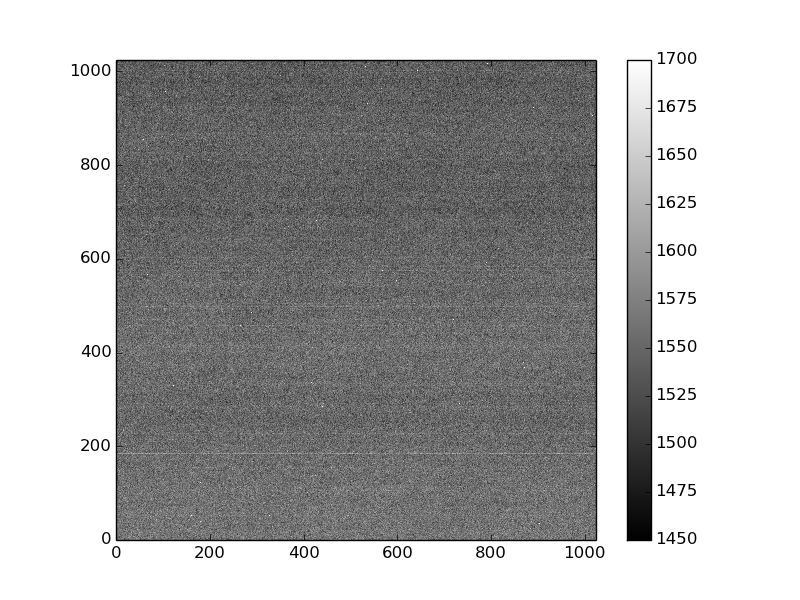
\includegraphics[scale=0.5]{figure_1}
\caption{\small Shows the average bias of the Apogee Alta U47 CCD used. The sidebar shows the count value by the intensity of gray. With this bias image it is obvious that even with a 0.00 second exposure the CCD still gives counts detected. This Average bias was acquired by taking ten separate biases and averaging the counts in the images. The median counts for the image = 1552 counts. This shows that images taken with this CCD must take into account the bias and subtract it from the raw images to get the true images.}
\end{figure}
\end{center}

\begin{center}
\begin{figure}[!hb]
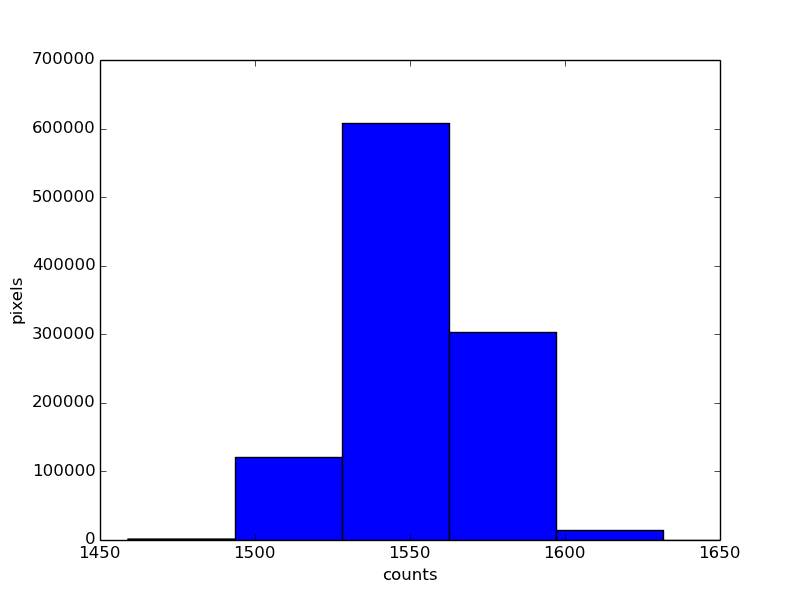
\includegraphics[scale=0.5]{figure_2}
\caption{\small Histogram of the counts recorded in Figure 1. shows a median and mean around 1550 counts. If the CCD was capable of distinguishing between photoelectrons and any other electron then this bias would not be necessary.}
\end{figure}
\end{center}

\begin{center}
\begin{figure}[!hb]
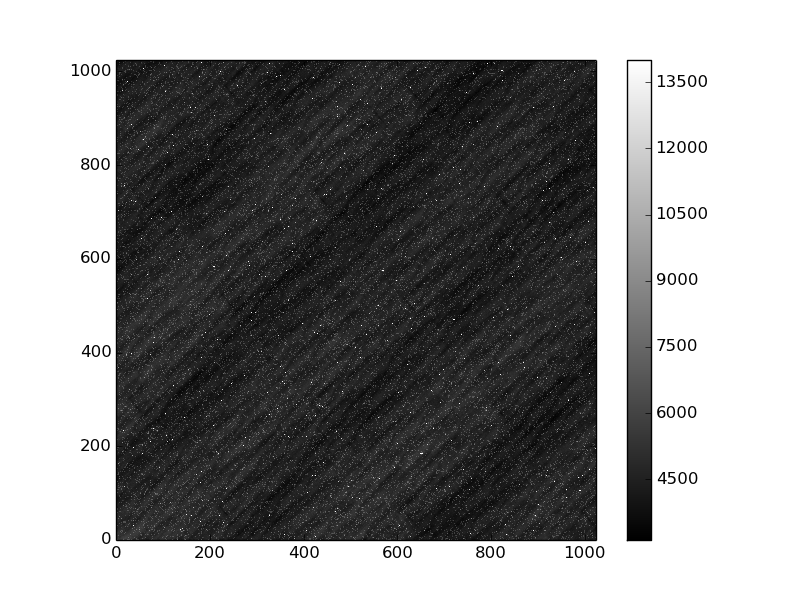
\includegraphics[scale=0.5]{figure_3}
\caption{\small electrons counted due to thermal motions of detector  at room temperature. The sidebar shows the count value by the intensity of gray.The counts are purely temperature dependent and can be easily seen when comparing the value to Figure 4. The mean counts at room temperature =  4708 $\pm$1149 counts.}
\end{figure}
\end{center}

\begin{center}
\begin{figure}[!hb]
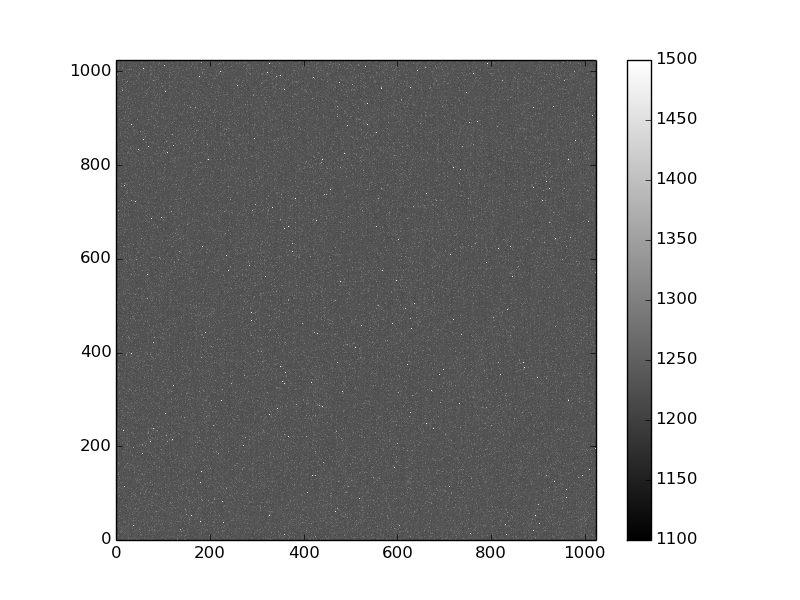
\includegraphics[scale=0.5]{figure_4}
\caption{\small The same experiment as Figure 3 with the exception of the detector in the CCD being cool down to  $-20\,^{\circ}{\rm C}$. The sidebar shows the count value by the intensity of gray. The mean counts for this dark image =1235  $\pm$ 41 counts.}
\end{figure}
\end{center}
 
\begin{center}
\begin{figure}[!hb]
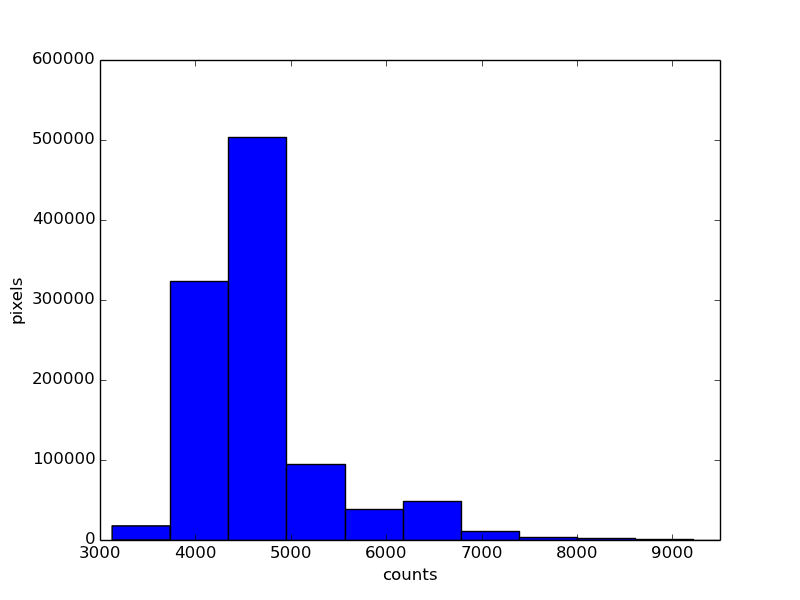
\includegraphics[scale=0.5]{figure_5}
\caption{\small Shows a histogram of the image in Figure 3. This shows where the mean and median are graphically. median = 4531, mean = 4708 $\pm$1149 counts. }
\end{figure}
\end{center}

\begin{center}
\begin{figure}[!hb]
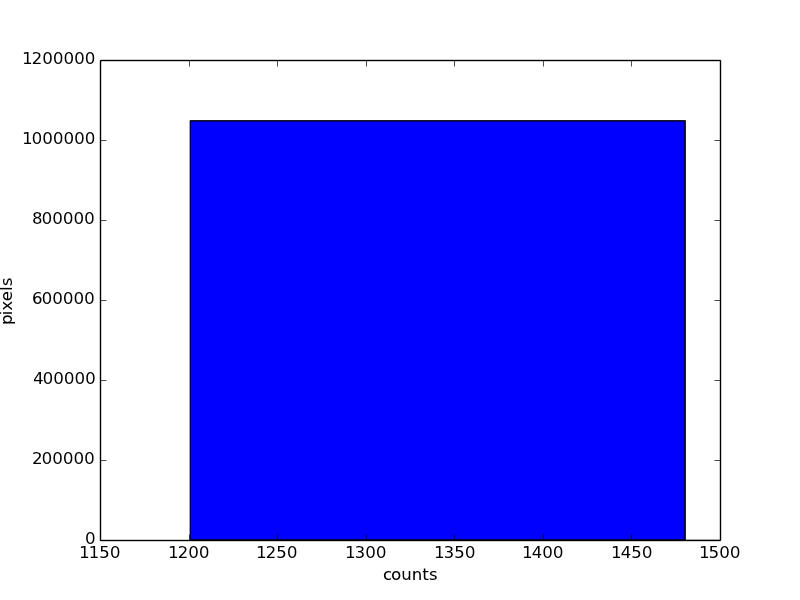
\includegraphics[scale=0.5]{figure_6}
\caption{\small Shows a histogram of the image in Figure 4. This shows where the mean and median are graphically. median = 1232, mean = 1235  $\pm$ 41 counts. This shows that dark currents in a CCD are directly dependent on temperature of the detector. The colder the detector is cooled the less dark current to account for making imaging much easier. This CCD is only cooled to $-20\,^{\circ}{\rm C}$, then CCD's cooled by liquid Nitrogen as is used in much more expensive telescopes have much smaller Dark Currents.}
\end{figure}
\end{center}

\begin{center}
\begin{figure}[!hb]
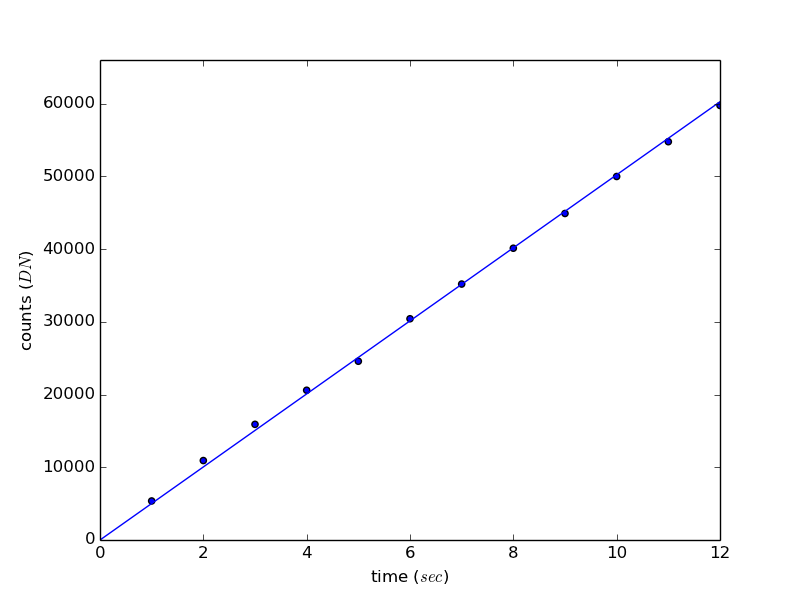
\includegraphics[scale=0.5]{figure_7}
\caption{\small  Shows a linear relationship between exposure time of the CCD and how many counts are recorded. With the Illumination level chosen the pattern remains linear up to around 20000 counts where the number of counts drops below the trend line. This is very useful because knowing the counts of a certain time exposure image, simple multiplication can be applied to get a target count number. The particular relationship for this level of illumination is approximately 4899 counts per second of exposure.}
\end{figure}
\end{center}

\begin{center}
\begin{figure}[!hb]
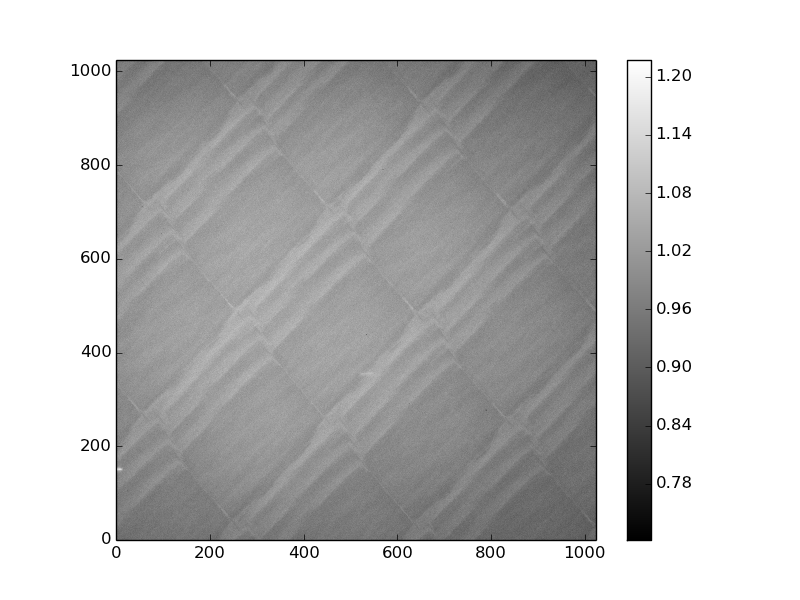
\includegraphics[scale=0.5]{figure_8}
\caption{\small Shows a normalized image where the highest value on the side bar represents the most counts. This shows the Quantum Efficiency of each pixel with side-by-side comparison. For this image the typical pixel variation is approximately 10\% which is larger than preferable. }
\end{figure}
\end{center}

\begin{center}
\begin{figure}[!hb]
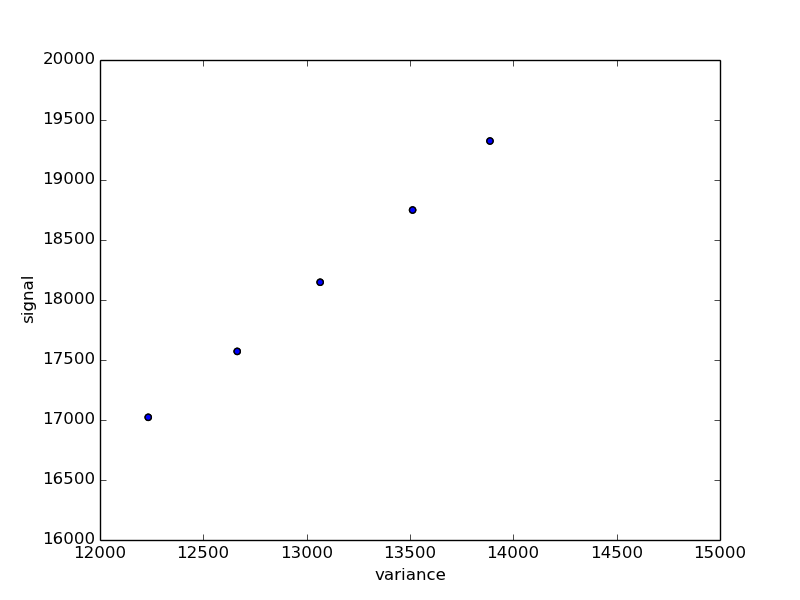
\includegraphics[scale=0.5]{figure_9}
\caption{\small Shows data points in a linear pattern representing the gain. The gain is quoted as being electrons per count in the CCD. The gain is calculated as variance as a function of signal. The gain is represented by $g$ = $\frac{N_{DN}}{\sigma^2_{DN}}$, g= 1.3862678 electrons/count in this experiment. This says that the number of electrons to reach saturation of an image is 65,535 $\cdot$ g = 65,535 $\cdot$ 1.3862678 = 90,849 electrons detected at saturation. any more electrons per pixel would begin spilling over into other pixels, so it is advised to stay well below this many electrons counted.}
\end{figure}
\end{center}

\begin{center}
\begin{figure}[!hb]
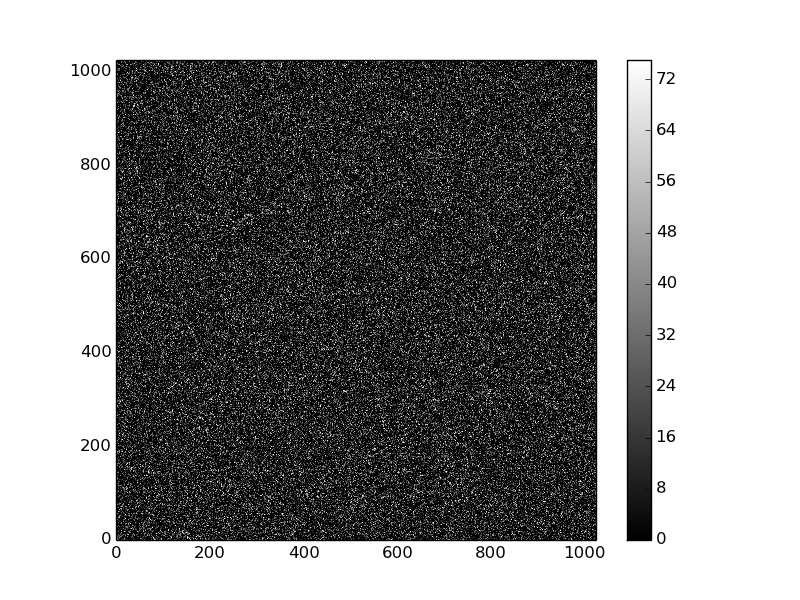
\includegraphics[scale=0.5]{figure_10}
\caption{\small Shows the read noise of every image recorded by this CCD. The read noise is a fixed pattern that can easily be discarded by taking the difference between two bias images. This leaves variations in the image caused by read noise. The read noise is calculated as $RN$ = $\frac{g *  \sigma_{\Delta B}}{\sqrt{2}}$ the value for the read noise is RN = 0.034915 }
\end{figure}
\end{center}

\begin{center}
\begin{figure}[!hb]
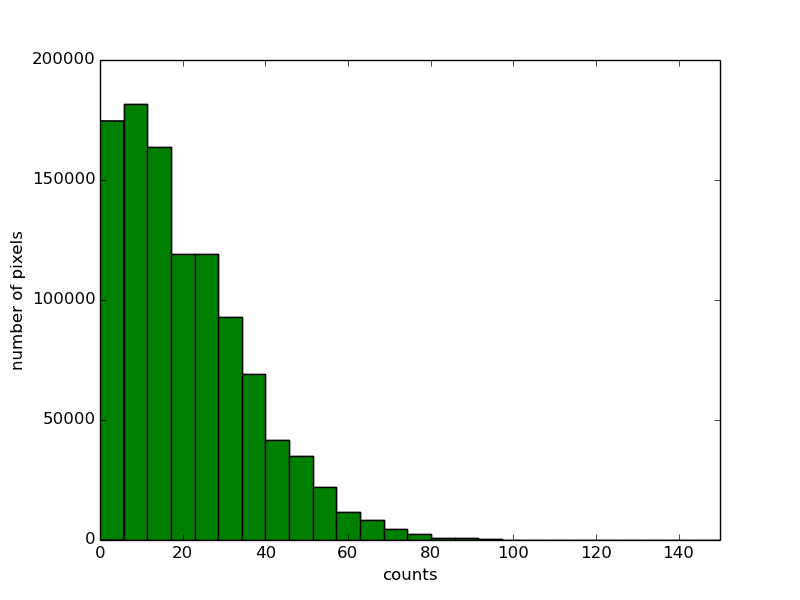
\includegraphics[scale=0.5]{figure_11}
\caption{\small shows graphically that the read noise of most pixels is small for most but still must be accounted for. Most pixels only have a few read noise counts but not taking them into account will skew results in any experiment done by this CCD.}
\end{figure}
\end{center}



\end {document}